\documentclass[11pt]{article}

\usepackage{a4wide}
\usepackage{mathptm}
\usepackage{xspace}
\usepackage{amsmath}
\usepackage{graphicx}
\usepackage{algorithm}
\usepackage{algpseudocode}
\usepackage{tikz}
\usepackage{tkz-graph}
\usetikzlibrary{shapes.misc, positioning}
\usepackage{listings}
\usepackage{color}
\usepackage{hyperref}
\usepackage{tabularx}
\usepackage{array}
\usepackage{subcaption}

\definecolor{dkgreen}{rgb}{0,0.6,0}
\definecolor{gray}{rgb}{0.5,0.5,0.5}
\definecolor{mauve}{rgb}{0.58,0,0.82}

\lstloadlanguages{C,C++,csh,Java}

\lstset{frame=tb,
  language=Java,
  aboveskip=3mm,
  belowskip=3mm,
  showstringspaces=false,
  columns=flexible,
  basicstyle={\small\ttfamily},
  numbers=left,
  numberstyle=\tiny\color{gray},
  keywordstyle=\color{blue},
  commentstyle=\color{dkgreen},
  stringstyle=\color{mauve},
  breaklines=true,
  breakatwhitespace=true,
  tabsize=3
}
\begin{document}

\title{Software Technology Project}

\author{Adrian Hatlenes Blikås, Andreas Øihaugen, Stian Sletvold Eilertsen and Thorbjørn Petter Melheim}

\maketitle

\begin{abstract}
  This project focuses on developing a prototype for a polling system designed to demonstrate the use of different technologies throughout the application. 
  The system provides a web-based interface for users and a REST API that gives the possibility of both external application use and also for the web-based interface, with secure access through user authentication. 
  The main objective was to create a functional solution that addresses core requirements and also utilize the framework for evaluating software technology. 
  The prototype is containerized using Docker, enabling deployment across environments. 
  Data is managed using PostgreSQL and MongoDB for storage. 
  The back end is implemented using .NET Core, while the front end uses a single-page application framework Svelte.
  This report details the design, technology choices, implementation, and results of the project.
\end{abstract}

\newpage
\tableofcontents
\newpage

%\input{commands}

\section{Introduction}
\label{sec:introduction}

This project focuses on the development of a full-stack prototype for a polling system. 
The goal was to design a system that is not only functional and secure but also capable of meeting the following key requirements:
\begin{itemize} 
    \item A web-based user interface with a REST API for external interactions. 
    \item Secure user authentication for controlled access. 
    \item Messaging broker.
    \item A database for structured data storage. 
    \item A database for unstructured data storage. 
\end{itemize}
The system incorporates various technologies to achieve these objectives. 
Initially, the project was set to use Spring Boot for the backend. 
However, one of the project goals was to explore alternative technology and utilizing the brown framework for evaluating software technology\cite{brown:96}. 
Therefore, we chose to use .NET Core with Entity Framework, enabling a change in the ORM giving us the opportunity to try the brown framework on ORM. 
The .NET Core framework supports REST API development, and Entity Framework, as the ORM. As some group members had used .NET as REST API in previous work this seemed to offer a feasible development timeline for the revised stack when compared to the course's compulsory assignment choice of Spring Boot and Spring JPA.
For the frontend, we implemented a single-page application using Svelte. 
Data storage was handled using two databases: PostgreSQL for structured data and MongoDB for unstructured data.
RabbitMQ is used for messaging and a stand alone Spring Boot application is retrieving the data from RabbitMQ and storing it in our MongoDB.
Containerization was implemented using Docker, with images hosted on Docker Hub to facilitate deployment.
The results indicate that the system meets its objectives by providing secure user access, effective data management, and seamless component integration. 
This report discusses the design process, the rationale behind key technology choices, the implementation details, and the outcomes, demonstrating the system’s ability to function as a robust and secure polling platform.\\
The report is organized as follows: \\
Section~\ref{sec:design} describes the system's design, including the architecture and use cases. \\
Section~\ref{sec:technology} outlines the selected technologies and their roles in the project. \\
Section~\ref{sec:implementation} explains the implementation process, and Section~\ref{sec:conclusions} discusses the outcomes and areas for improvement.\\
\noindent
The custom docker images can be found \cite{noauthor_h598970dat250_api_nodate} and \cite{noauthor_h598970dat250_messaging_nodate}. \\
The complete project can be found here \cite{github_598975project-restapi_nodate}, \cite{github_thorbjorn2021project-messaging_nodate} and \cite{github_598975project-frontend_2024}.



\section{Design}
\label{sec:design}

Around 5 pages about functional aspects of the FeedApp application.

Concretely, you shall write about 

\begin{itemize}
	\item the \emph{use cases},
	\item the \emph{domain model}, and
	\item the \emph{architecture} (including applied technologies)
\end{itemize}

Each part shall ideally be accompanied with a graphical representation (diagram).

You may have a look at the \href{https://github.com/selabhvl/dat250public/blob/master/projectdescription/README.md}{Examples on GitHub}.




\subsection{Use cases}

The purpose of a use case diagram is to outline the functionalities the system will implement, identify the various roles involved, and specify where user interfaces are needed. The UML provides a high-level view of system interactions which features are necessary, who will be using them, and how users will access them within the application. 

In the FeedApp application is there two separate roles. First there is the anonymous user. An anonymous user can only view and vote on public polls. They can also register a new account or log in to an existing one. A logged in user can view and vote on every poll. The logged in user can also create a new poll or edit and delete their existing polls.

\begin{figure}[thb]
	\centering
	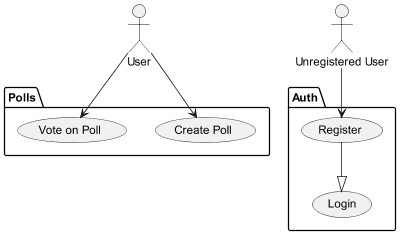
\includegraphics[scale=0.5]{figs/PUML/UseCase.png}
	\label{fig:Use cases}
\end{figure}

Poll availability is decided by the polls author upon creation. 

\subsection{Domain model}

The domain model shows the domain concepts and their relations. A user can have several votes and polls. Each poll have one user who created the poll and two or more poll options. Each of the poll options can have several votes. 

\begin{figure}[thb]
	\centering
	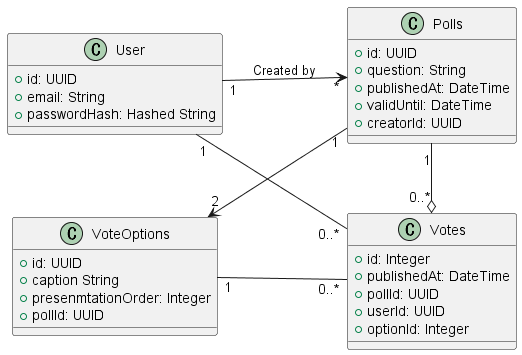
\includegraphics[scale=0.5]{figs/PUML/DomainModel.png}
	\label{fig:Domain model}
\end{figure}

\subsection{System architecture}

For the desing of the FeedApp and the analytic components are several technologies needed. The figure shows the different parts of the app and the technologies used to implement them. For the frontend is Svelte used. 

For the backend is ASP.NET Core used. 


\begin{figure}[thb]
	\centering
	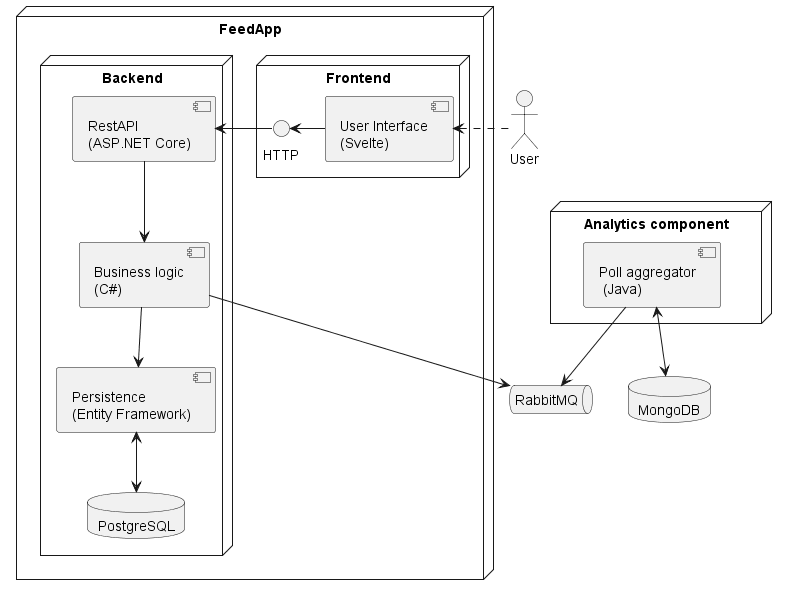
\includegraphics[scale=0.5]{figs/PUML/SystemArchitecture.png}
	\label{fig:System architecture}
\end{figure}



\section{Technology Assessment}
\label{sec:technology}


Introduce in (sufficient) depth the key concepts and architecture of the chosen software technology. As part if this, you may consider using a running example to introduce the technology.

This part and other parts of the report probably needs to refer to
figures. Figure~\ref{fig:framework} from \cite{brown:96} just
illustrates how figure can be included in the report.

Entity Framework (EF) is an Object-Relational Mapper (ORM) developed by Microsoft for the .NET platform. An ORM supports the creation of applications focused on data management by abstracting the data storage and allows developers to focus on the business logic of their applications while interacting with underlying databases. This abstraction reduces the need to write extensive boilerplate code for database operations and provides a more intuitive object-oriented approach to data handling.

Entity Framework does this by dividing the application into three parts: the conceptual model, the storage model, and the mappings between them. The conceptual model represents the application's domain entities and relationships. It abstracts the data source, allowing developers to work with objects and relationships at a higher, business-oriented level. The storage model describes the logical structure of the database, including tables, columns, keys, and constraints. This model is specific to the underlying data source. Developers interact primarily with the conceptual model, making the application independent of the specific database technology. The Mapping specification language (MSL) defines the mappings between these two models, which specifies how entities, properties, and relationships in the conceptual model align with the database schema in the storage model. The conceptual model is defined using classes in code, and configurated to specify how these classes should be connected in the database.  

\begin{figure}[thb]
	\centering
	\includegraphics[scale=0.5]{figs/framework.png}
	\caption{Software technology evaluation framework.}
	\label{fig:framework}
\end{figure}

\subsection{Descriptive Modeling}

write where the technology comes from, its history, its context and what problem it solves.
Consider drawing a graph like in \cite{brown:96}.

\textbf{Technology genealogy}
The first version of Entity Framework was released in 2008, as part of .NET Framework 3.5 SP1 and Visual Studio 2008 SP1, by Microsoft. Prior to EF, developers relied on ADO.NET for data access within .NET applications. Entity Framework (EF) was developed as an answer to two different objectives, to raise the level of abstraction when working with modelling of entities, and data engines to store and retrieve data. EF enables developers to work with data in the form of domain-specific objects and properties, such as customers and customer addresses, without having to concern themselves with the underlying database tables and columns where this data is stored. With EF, developers can work at a higher level of abstraction when they deal with the data and can create and maintain data-oriented applications with less code than in traditional applications [1]. Its first version was widely criticized, even attracting a “vote of no confidence” signed by at least one thousand developers [3]. The second version, EF 4.0, was as part of .NET 4.0 in 2010 and addresses many of the criticisms made of version 1, such as lazy loading, testability improvements, foreign key mapping, support for Plain old CLR object (POCO) which is a simple object created in .NET, often used in opposition to complex or specialized objects that object-relational mapping framework often require [5].  With the release of version 6.0 in 2013, EF became an open source project licensed under Apache License v2. With this version, EF was also moved out of the band from the .NET Framework, which helps in accelerating the pace of development and delivery of new features [4]. 


\subsection{Experiment Design}
\label{subsec:experiment_design}
Keeping in line with our evaluation framework \cite{brown:96} we are to first do a comparative feature analysis before we further our attention towards creating hypotheses and experiment design.
To start of our experiment design we create a comparative feature analysis.

\subsubsection{Comparative feature analysis}
To conduct our comparative feature analysis we created Table~\ref{tab:jpa_vs_ef_vs_no_orm}, in this table we have looked at the official documentation of the Entity Framework \cite{ef_getting_started} and the official documentation of JPA \cite{spring_jpa}.
\begin{table}[H]
    \centering
    \begin{tabularx}{\textwidth}{|l|X|X|X|} % Define column widths with borders
        \hline
        \textbf{Feature} & \textbf{JPA} & \textbf{Entity Framework} & \textbf{Not Using ORM} \\ \hline
        Schema Abstraction & Relies on annotations and configuration (e.g., Hibernate supports @Table, @Column). & Strong tooling with migrations (Add-Migration, Update-Database commands). & Schema directly defined and managed in SQL scripts or database-specific tools. \\ \hline
        Schema Evolution Tools & Schema auto-generation and validation with support for tools like Flyway and Liquibase. & Built-in migration system for versioning and rolling back schema changes. & Requires manual management of schema changes and evolution. \\ \hline
        Query Abstraction & JPQL for writing abstract, database-independent queries. & LINQ provides strongly-typed, language-integrated query capabilities. & Direct SQL queries must be written and maintained, often specific to the database. \\ \hline
        CRUD Boilerplate Reduction & Automatic through frameworks like Spring Data JPA. & Automatic using EF Core Repositories and DbContext for basic CRUD operations. & No automation; full CRUD operations must be manually implemented in SQL or procedural code. \\ \hline
        Ease of Refactoring & Code annotations simplify model changes but may require manual migration scripting. & Strong support through auto-generated migration files and IDE integration. & Refactoring requires careful updates to SQL scripts and application code to avoid inconsistencies. \\ \hline
        Cross-Platform Support & Platform-agnostic via the JVM, supports multiple database engines. & Cross-platform with .NET Core but optimized for Windows and SQL Server. & Fully dependent on the database and programming environment used. \\ \hline
        Code Complexity Reduction & Annotations reduce code overhead for mappings but require verbose configuration files. & Strongly-typed models and DbContext minimize configuration and boilerplate code. & High complexity due to explicit SQL queries and manual schema synchronization. \\ \hline
    \end{tabularx}
    \caption{Comparison of JPA, Entity Framework, and Not Using ORM}
    \label{tab:jpa_vs_ef_vs_no_orm}
\end{table}


As shown in Table \ref{tab:jpa_vs_ef_vs_no_orm} we see that there are some clear similarities and some differences. 
As a proper first step we wanted to focus our attention on ORM´s contribution to a project like our own.
This helped us generate the hypotheses found in the next section.

\subsubsection{Hypotheses}
Looking at the ORM's we could see that what we could call programmer comfort is an important part of what the ORM's contribution to the project. 
Another important part looks to be the reduction of repetitive or "boilerplate" code.
With this in mind we created the following hypotheses:

\textbf{Hypotheses one} \newline
The abstraction provided by an ORM simplifies maintenance and refactoring of database schemas. \\

\textbf{Hypotheses two} \newline
ORM shortens development time by reducing unnecessary boilerplate code. \\

We believe these hypotheses would give an interesting insight regarding the possible benefits of utilizing an ORM.

\subsubsection{Experiment design}
As the name of the subchapter \ref{subsec:experiment_design} hints to we are to design an experiment. 
To test our hypotheses we want to create some experiments that are possible to recreate and that are measurable. \\

\textbf{Experiment for hypotheses one} \\
To test if an ORM simplifies maintenance and refactoring of database schemas we need to simulate schema evolution scenarios in ORMs and without ORM.
To be certain that the experiment is measuring the correct parameters we want to make sure that the database technology is the same and in our case that means using PostgreSQL, and we also want to make the same changes to the table in all experiments.
To measure the differences we want to look at the following: 
\begin{itemize}
    \item Measure the time it takes to apply schema changes.
    \item Developer effort (lines of code modified, complexity of changes)
    \item Risk of introducing errors (While timing the schema change time also record any breaking changes)
\end{itemize}


\textbf{Experiment for hypotheses two}
To test if an ORM shortens development time by reducing unnecessary boilerplate code we need to build a CRUD application.
To be certain that the experiment is measuring the correct parameters we need to have some controlled variables like all applications needs to have the same functional requirement.
To measure the differences we want to look at the following:
\begin{itemize}
	\item Development time.
	\item Code size
	\item Complexity and readability (measured by developer feedback)
\end{itemize}

\subsection{Experiment Evaluation}
The experiment evaluation face we are sectioning into setup, methodology, results, discussion and limitations.\\
The experiments for both hypotheses as outlined in the previous subsection \ref{subsec:experiment_design} the fist hypotheses is dependent on a completed project and the second is largely dependent on creating a project.
These dependencies give us the opportunity to combine the valuation experiments into one experiment.
The experiment evaluates how ORM frameworks (JPA and EF) \textbf{impact development time}  and \textbf{schema maintenance}.\\ 
The hypothesis states that ORM abstraction:
\begin{enumerate}
	\item ORM abstraction simplifies schema maintenance compared to raw SQL.
	\item ORM reduces development time by minimizing repetitive code.
\end{enumerate}

\subsubsection{Experiment setup}
We want to assess CRUD implementation and schema maintenance efficiency for JPA, EF Core and raw SQL.

\textbf{Environment} \\
We want the environments to be as similar as possible, but some differences are present.
\begin{itemize}
	\item PostgreSQL is used for all applications.
	\item For EF Core Visual Studio 2022 is used.
	\item For JPA IntelliJ IDEA is used.
\end{itemize}

\textbf{Database model}
The database schema needs to be the same for all applications.
\begin{verbatim}
	Poll(ID, Question, PublishedAt, ValidUntil, VoteOptions)
	VoteOption(ID. Caption, PresentationOrder)
\end{verbatim}

\textbf{Tasks} \\
The experiment is to be conducted by implementing CRUD operations for Poll and VoteOption.
When the CRUD operations are implemented \textbf{Title} is to be added to \textbf{Poll}.

\subsubsection{Methodology}
Due to constraints of time the experiment involves only one developer.

\textbf{Metrics} \\
We measure the following:
\begin{itemize}
	\item \textbf{Development Time}: Time to complete each task.
	\item \textbf{Lines of Code (LOC)}: To quantify boilerplate reduction.
	\item \textbf{Error Rate}: Number of runtime errors encountered during task completion.
\end{itemize}

\textbf{Process} \\
\begin{itemize}
	\item The developer is timed while implementing CRUD operations and performing the schema modification.
	\item Errors are logged, and corrections incur time penalties.
	\item Tasks are executed in a consistent environment to minimize external influences.
\end{itemize}

\subsubsection{Results}
\textbf{Development Time} \\
\begin{tabular}{|l|c|c|c|}
\hline
\textbf{Task} & \textbf{JPA (Hibernate)} & \textbf{EF Core} & \textbf{Raw SQL} \\ \hline
CRUD Operations & 45 min & 30 min & 60 min \\ \hline
Schema Modification & 25 min & 5 min & 40 min \\ \hline
\end{tabular}

\textbf{Lines of Code (LOC)} \\
\begin{tabular}{|l|c|c|c|}
\hline
\textbf{Task} & \textbf{JPA (LOC)} & \textbf{EF Core (LOC)} & \textbf{Raw SQL (LOC)} \\ \hline
CRUD Operations & 120 & 90 & 200 \\ \hline
Schema Modification & 30 & 20 & 60 \\ \hline
\end{tabular}

\textbf{Error Rate} \\
\begin{tabular}{|l|c|c|c|}
\hline
\textbf{Task} & \textbf{JPA} & \textbf{EF Core} & \textbf{Raw SQL} \\ \hline
CRUD Operations & 2 & 1 & 4 \\ \hline
Schema Modification & 1 & 0 & 3 \\ \hline
\end{tabular}

\subsubsection{Discussion}
\textbf{Development Time} \\
EF Core demonstrated the shortest development time due to its integrated migration tools and LINQ support, which makes schema updates and query construction easier. JPA was similar in development time, but its annotation-based configuration added up to more time spent programming. Raw SQL required the most time, as every query and schema change had to be manually implemented.

\textbf{Lines of Code (LOC)} \\
EF Core had the least LOC due to its DbContext abstraction, reducing boilerplate code to what seems like a minimum. JPA required more lines due to annotations. Raw SQL added the most LOC due to requiring explicit query and schema manipulation logic.

\textbf{Error Rate} \\
EF Core had the lowest error rate, benefiting from compile-time checks for LINQ queries and Visual Studio debugging tools. JPA had slightly more runtime errors, as JPQL queries are validated at runtime. Raw SQL had the highest error rate due to manual query construction, which increased typos and logic errors.

\subsubsection{Conclusion}
The experiment shows that ORMs (EF Core and JPA) significantly reduce development time and boilerplate code compared to raw SQL. EF Core emerged as the most efficient ORM due to its tooling and abstraction, but JPA performed well in cross-platform scenarios. Raw SQL offers maximum control and may be preferable for performance-critical applications.



\section{Prototype Implementation}
\label{sec:implementation}

The project consists of three major parts that can be found in individual GitHub repositories. The front-end web interface built in Svelte, the REST-API back-end built in ASP.NET Core with EntityFramework Core, and the messaging service built in a Spring application. To run the project, clone the REST-API GitHub repository and launch the Docker container using the docker-compose.yml file.

\subsection{Back-end}

The back-end application repository which contains the built static files for the SPA and the Docker Compose file for the entire application can be found \href{https://github.com/598975/project-RESTAPI}{here on GitHub}.
\newline
\newline
The back-end REST API and business logic is built in C\# in the framework ASP.NET Core. The .NET project root contains default C\# project files which configure the settings and behavior of the project. A lot of this is standardized, but may need to be configured to match the needs for the project. For example, the appsettings.json file contains the connection string for connecting to the PostgreSQL database and the Program.cs file enables the use of ASP.NET Core authentication and tells the app to use static which are found in the wwwroot directory. 

The application uses the Model-View-Controller (MVC) design pattern. The models are contained in the Models directory. The models are classes which represent and defines the data entities of the application and equivalent to their respective tables in the database. Figure~\ref{fig:voclass} showcases the VoteOption class. You can here see the use of annotations to set the identifying key (primary key) for the class and for this key to be a auto incrementing integer.

\begin{figure}[hbtp]
    \caption{The VoteOption class}
	\centering
	\begin{lstlisting}[language=csh]
    public class VoteOption
    {
        [Key]
        [DatabaseGenerated(DatabaseGeneratedOption.Identity)]
        public int Id { get; set; }
        public String? Caption {  get; set; }
        public int PresentationOrder { get; set; }
    }
    \end{lstlisting}
	\label{fig:voclass}
\end{figure}

Controllers are contained in the Controllers directory. Annotations are used for specifying that the classes are controllers, authorization, routing and for what type of HTTP method a function is. The functions are generated but edited to fit the needs of the application. An important functionality for the controllers is the AppDBContext class (in the Data directory) which extends the Entity Framework Core IdentityDbContext class. This is used to query the database for objects and for saving changes to the database.

\subsection{Front-end}

The code behind the built static front-end files can be found in the \href{https://github.com/598975/project-frontend/tree/main}{projects front-end} repository on GitHub. W3CSS is used for styling the application \cite{W3CSS}.
\newline
\newline
The front-end part of the application is built in Svelte with JavaScript. It consists of a SPA which uses the JavaScript Fetch API to interact with the back-end parts of the application. In the finished application the static files JavaScript, CSS and HTML files have been built with the npm command \verb|npm run build| and moved into the back-end. It can however also be ran as a standalone application using the command \verb|npm run dev|. 

During development prior to building the finished front-end, the back- and front-end applications were ran separately. Proxies have been added to the vite.config.js file in order for the front-end to communicate with the back-end with simpler addresses. In the finished application the back- and front-end were combined as this requires fewer processes running concurrently and because running them separately weakens security as it requires weaker Cross Site Request Forgery (CSRF) protection.

The file App.svelte handles the routing of the components/templates in the application. The file Authorization.svelte is used to check if the session is authorized by fetching the /pingauth endpoint from the REST API which return the email of the logged in user if a user is logged in. If not, it show the login template. The templates directory contains the different unique templates that can be shown. The Index template is the default template you will be routed to. If authorized, it will display all existing polls and allow you to create new polls or vote on existing ones. These operations are handled and defined in the Polls.svelte file in the libs directory.


\subsection{Messaging and NoSQL storage}

The main portion of the messaging parts of the application can be found in the \href{https://github.com/Thorbjorn2021/project-Messaging/tree/main}{messaging repository} on GitHub.
\newline
\newline
An aggregated view of the polls is stored in a MongoDB database. Sending these views to the database is done by using the messaging broker RabbitMQ. The RabbitMQ broker and the analytics component uses Java business logic and is built in a Spring application. 

The client that publishes messages is implemented in the RestAPI in the class RabbitmqClient.cs in the Messaging directory. The VotesController uses this class to publish a message whenever the Post request is triggered, which is whenever any authorized user votes on a poll.

The broker server is active in the background checking for new messages. Whenever it detects a new message in the message queue, it recieves this message, retrieves its contents and save them to the MongoDB database. Recieving the messages is handled by the Reciever.java class and saving the aggregated polls to the database is handler by the AggregatedPollRepository.java class.

\section{Conclusions}
\label{sec:conclusions}

The concluded project is a functioning demo of the application described in the problem description. 
The various different technologies function together without any conflicts. 
The result of the project is not a complete and finished application, and it would require additional features and changes to reach a point where it could be used as a finished product, but it still manages to showcase the chosen technologies.
Some missing features are for example giving people access to voting when not logged in. This would be a functionality that we would expect from a voting system like this. We would also expect there to be some way of accessing the analytical data from votes in a dashboard. These are just some features we would recommend adding to the application.
To summarize the technology chosen both EF Core and framework ASP.NET Core have been simple both to learn and work with. 
The official documentation is thorough and extensive \cite{EFoverview}, and the experiments in section \ref{sec:technology} showcase the development speed the framework allows. 
The syntax of the framework and reduction in boilerplate code has lead to code that is easy to understand and read.
The rest of the stack has been interesting working with and adapting to our project so that we have a functional applicaton.
Looking at our work with the framework for evaluating software technology we have seen that as with all frameworks applying it to the real world and using it is the only way of learning it.
After using a sizable sum of time trying to understand the framework and doing and redoing the analysis it is easy to see that the next time it would be easier and perhaps yield more tangible results in future applications.


\addcontentsline{toc}{section}{References}
\bibliographystyle{plain}
\bibliography{report.bib}{}

\end{document}
